\chapter{Spatial-cell}
\label{chap:spatial-cell}

In spatial model, the concentration is defined based on the volume of a single
grid point, i.e. $V_\myo$ not $V_\myoT$, and $V_\nsr$ not $V_\nsrT$. As a
result, there is no change in $[\Ca]_\myo$ and $[\Ca]_\nsr$ for a single grid
point. The major point is the balance equation, defined in
Sect.\ref{sec:balance-eq_spatial}. The second point to notice is the fluxes,
where the transfer rate is defined differently,
Sect.\ref{sec:transfer_rate-spatial}. The third point is the bacground
conductance $g_\bCa$, which is now defined based on which reference volume being
used.

\begin{itemize}
  \item From main.f95:
\begin{enumerate}
\item Read in parameter file \verb!prog_get_info()! 
\item Validate data from parameter file \verb!check_ecc_data()! 
\item Initialize GPU to use \verb!init_GPU(gpuID)! 
  (\textcolor{red}{we may need to remove this function and the
    command-line argument when multiple GPUs is implemented})
    
\item \sout{Make compact Ks matrices} \verb!makecompKs2_T()! and
\verb!makeKs_nj_6_2!. \sout{To deal with a general case: we use}
\verb!makecompKs3_T()!.
 
\item Call \verb!setup_RyR()! and \verb!setup_LCC()! which works for any 
Markov-based models using certain functional transition rate (i.e.
$[\Ca]_\ds$-dependent activation, $V_m$-dependent
activation/inactivation\ldots).

\begin{framed}
The non-transpose forms are used from now on, as there's no difference in
performance between transposed and non-transposed forms.
\end{framed}

\item For non-junctional RyR:
\begin{enumerate}
  \item \sout{If we consider non-junctional RyRs as explicit clusters: we call}
  \verb!makecompKs_RyRsmall_T! (or \verb!makecompKs_RyRsmall!)
  (Chap.\ref{chap:small_RyR_cluster}).
  \item \sout{If we consider non-junctional RyRs as homogeneous clusters, i.e.
  equally distribute the contribution to every grid points:}
  we call \verb!makeKs_nj_7_2! or \verb!makeKs_nj_6_2()!.
  \item we call \verb!makeKs_nj()!. 
\end{enumerate}
   
\item Initialize data for simulation \verb!init_Simulation()!
(Sect.\ref{sec:spatial_init_simul})
\item Run simulation \verb!continue_Simulation()! (Sect.\ref{sec:continue_simulation})
\end{enumerate}
  
  \item From tscell\_utility.f95: contains
  \begin{enumerate}
    \item \verb!init_Simulation()!
    \item \verb!continue_Simulation()!: call \verb!simulate_NextSteps()!.
    \item \verb!simulate_NextSteps()!: Sect.\ref{sec:simulate_nextsteps}
  \end{enumerate}
\end{itemize}

\section{init\_Simulation}
\label{sec:spatial_init_simul}

  \begin{enumerate}
    \item Allocate on GPU to copy compact Ks matrices to there
    (Sect.\ref{sec:Ks_compact}).
	\item Allocate non-spatial GPU data (Sect.~\ref{sec:gpu-data}) and CPU data
    (Sect.~\ref{sec:cpu-data})
    \item Load data \verb!loaddata_from_conf()!,
    \begin{itemize}
    \item Init CaRU state \verb!init_SFU_State()!
    \item Init ECC data \verb!init_data_ECC()!
    \item Init Fluorescence data at resting \verb!init_Fluo()!
      (Sect.~\ref{sec:fluorescence})
    \end{itemize}

  \item If continue a previous simulation, then evoke
    \verb!loaddata_from_restartfile()! to read from restart file;
    
    else evoke \verb!init_SpatialCell()! to init cell (Geometry + Data)
    (Sect.~\ref{sec:spat-cell-geom})
  
  
  \item Init PRNG \verb!init_PRNG()! \item Setup kernel
  \verb!setup_KernelConfiguration()! (Sect.\ref{sec:kernel-setting}) \item
  Initialize data for I/O \verb!data_io_init()! \item Copy to constant memory
  \verb!set_device_constant()!
  \end{enumerate}


\subsection{Compact form Ks matrices}
\label{sec:Ks_compact}

The zero-th column of \verb!idxK...! matrices keep the value that tell number of
non-zero elements in each column. The zero-th column of \verb!compK...! matrices
are always zero. 
\begin{verbatim}
    ALLOCATE(compKv1_dev(0:maxnkv1, NUM_STATES_SFU) &
         ,compKv2_dev(0:maxnkv2, NUM_STATES_SFU), compKm1_dev(0:maxnkm1, NUM_STATES_SFU) &
         ,compKm2_dev(0:maxnkm2, NUM_STATES_SFU), compKp1_dev(0:maxnkp1, NUM_STATES_SFU) &
         ,compKp2_dev(0:maxnkp2, NUM_STATES_SFU), STAT=iserror)

    ALLOCATE(idxKv1_dev(0:maxnkv1, NUM_STATES_SFU), &
         idxKv2_dev(0:maxnkv2, NUM_STATES_SFU), idxKm1_dev(0:maxnkm1, NUM_STATES_SFU), &
         idxKm2_dev(0:maxnkm2, NUM_STATES_SFU), idxKp1_dev(0:maxnkp1, NUM_STATES_SFU), &
         idxKp2_dev(0:maxnkp2, NUM_STATES_SFU), STAT=iserror)
\end{verbatim}


\subsection{Spatial data}
\label{sec:spatial_data}

To transfer data between GPU and CPU, we use a single pair of variables
allocated on page-locked memory
\begin{verbatim}
ts_data3D
ts_data_lin
\end{verbatim}

We also generate a number of linearized memory variables to store data, mainly
for initial setting, or when first copying them to GPU from CPU in the beginning
of the simulations
\begin{verbatim}
ts_Ca_myo_lin(SIZEWITHBOUNDARY)
ts_Ca_nsr_lin(SIZEWITHBOUNDARY)
ts_CaF_lin(SIZEWITHBOUNDARY)
\end{verbatim}



\subsection{Non-spatial data}
\label{sec:non-spatialdata}

\subsubsection{GPU data}
\label{sec:gpu-data}

GPU data from non-spatial model 
\begin{lstlisting}
// calcium
Ca_ds_dev (0:NSFU)
Ca_jsr_dev (0:NSFU)

// fluxes
J_efflux_dev (0:NSFU)
J_refill_dev (0:NSFU)
J_ryr_dev (0:NSFU)

// LCC current
I_dhpr_dev (0:NSFU)      --can derive--> J_dhpr


// current number of open channels
RyRgate_dev(NSFU)
DHPRgate_dev(NSFU)

// # open channels in all states
U_Ro_dev(NUM_STATES_SFU)
U_Lo_dev(NUM_STATES_SFU)

// keep rate transition of state unchanged
compPdt_dev(NSFU,1)

X_r_dev(NSFU*copy_interval)
\end{lstlisting}

NOTE: \textcolor{red}{We need to add the 0-th index element and asign it
to zero (0.0d0) as this one will be used in spatial mapping}
(Sect.\ref{sec:spatial-data}).


\subsubsection{CPU data}
\label{sec:cpu-data}


CPU data from non-spatial model. Data should reside on pinned memory if they are
used to contain the data copied back from GPU. 

\begin{lstlisting}
Ca_ds(NSFU)
Ca_jsr(NSFU)

// index of current state
sfu_state(NSFU)

RyRgate(NSFU)
DHPRgate(NSFU)

// fraction of channels in each nj states
p_nj

\end{lstlisting}




\subsection{Kernel setting}
\label{sec:kernel-setting}

NOTE: \textcolor{red}{Play with different configuration settings and see which
one works the best}
\begin{lstlisting}
#if _GPU_MODEL_ == _TESLA
  INTEGER, PARAMETER :: BLOCKSIZE_1D = 196
  INTEGER, PARAMETER :: BLOCK_DIMX = 32, BLOCK_DIMY = 8 ! 256 threads/block (Tesla)
#elif _GPU_MODEL_ == _FERMI  
  INTEGER, PARAMETER :: BLOCKSIZE_1D = 256
  !INTEGER, PARAMETER :: BLOCK_DIMX = 32, BLOCK_DIMY = 16 ! 512 threads/block (Fermi)
  INTEGER, PARAMETER :: BLOCK_DIMX = 64, BLOCK_DIMY = 8 ! 512 threads/block (Fermi)
  !INTEGER, PARAMETER :: BLOCK_DIMX = 32, BLOCK_DIMY = 8 ! 256 threads/block (Fermi)
  !INTEGER, PARAMETER :: BLOCK_DIMX = 16, BLOCK_DIMY = 16 ! 256 threads/block (Fermi)
#endif
\end{lstlisting}

1D thread-block, for kernels to update CRUs information
\begin{lstlisting}
    !for 1D thread BLOCK
    blocksize = BLOCKSIZE_1D
    gridSize = INT((NSFU+blocksize-1)/blocksize)  ! ceiling value
    !!gridSize = CEILING(REAL(NSFU)/blocksize)  ! ceiling value
\end{lstlisting}

2D thread-blocks, for kernel to update mesh-data information
\begin{lstlisting}
    dimBlock = dim3(BLOCK_DIMX, BLOCK_DIMY, 1)

#if _GRID_STRATEGY_ == _1THREAD_1ELEMENT
! Each layer/slice of the cell is put side-by-side into thread grid

!!!NOTE: only process inner cells (skip stencil cells for a
!!!separate kernels to update boundary values
    dimGrid = dim3(CEILING(REAL(outerDIMX) / dimBlock%x), & 
         CEILING(REAL(outerDIMY)/ dimBlock%y) * MAXZ, 1)
!!! this will be used for kernels to update boundary values
    dimGridStencil = dim3(CEILING(REAL(outerDIMX) / dimBlock%x), & 
         CEILING(REAL(outerDIMY)/ dimBlock%y), 1)
    
#elif _GRID_STRATEGY_ == _1THREAD_1DEPTHCOLUMN
    dimGrid = dim3(CEILING(REAL(outerDIMX) / dimBlock%x), & 
         CEILING(REAL(outerDIMY)/ dimBlock%y), 1)
!!! this will be used for kernels to update boundary values
    dimGridStencil = dim3(CEILING(REAL(outerDIMX) / dimBlock%x), & 
         CEILING(REAL(outerDIMY)/ dimBlock%y), 1)
#elif _GRID_STRATEGY_ == _1THREAD_1DEPTHCOLUMN_2OUTPUTS
    dimGrid = dim3(CEILING(REAL(outerDIMX) / dimBlock%x/2), & 
         CEILING(REAL(outerDIMY)/ dimBlock%y), 1)
!!! this will be used for kernels to update boundary values
    dimGridStencil = dim3(CEILING(REAL(outerDIMX) / dimBlock%x), & 
         CEILING(REAL(outerDIMY)/ dimBlock%y), 1)    
#endif    
\end{lstlisting}


\section{continue\_Simulation()}
\label{sec:continue_simulation}

\begin{lstlisting}
nsteps = copy_interval ! when to copy/generate new data (X_r_dev) to device

LOOPS until END
    data_io_print()
    call simulate_NextSteps(nsteps, is_EndSim)

    if (is_EndSim) return
ENDLOOP

!! writing the last time
CALL data_io_finalize()
\end{lstlisting}
The most important subroutine is \verb!simulate_NextSteps()!

\section{simulate\_NextSteps(nsteps)}
\label{sec:simulate_nextsteps}

The subroutine performs a number of simulation steps. $nsteps$ tells how often
the data is copied back from GPU to host for I/O.
\begin{lstlisting}
generate_random_numbers enough for nsteps iterations

ITERATE nsteps

*find the time step via 
  1. find Prob. of stay unchanged at all CaRUs
  2. min of these Prob.

*update new states + Cads + Cajsr

*update other ionic components (K1, Ktos, Ktof, Na...)

*udpate Camyo, Cansr

END ITERATION
\end{lstlisting}

\subsection{Find the time step}
\label{sec:time_step}

\begin{lstlisting}
#if _TEST_NEW_ORPHAN_CRU_ == _YES 
       CALL get_compPdt_3b <<<gridSize, blocksize>>> 
                   (kva, kvi, NSFU_normal, Ej_orphan, time)
#else
       CALL get_compPdt_3 <<<gridSize, blocksize>>> (kva, kvi, time)          
#endif
       cuErr = cudaThreadSynchronize()
       !!use min on GPU
       min_Pdt = min_reduce_double_2host(compPdt_dev(1:NSFU,1), NSFU, odata_d)

       dtmax =-0.1d0/min_Pdt
       dt = MAX(MIN(dtmax,dt_UB),dt_LB)
       
       time = time+dt
       invdt = 1.d0/dt
\end{lstlisting}

\subsection{Update new states for all CaRUs + Cajsr + Cads}
\label{sec:update_SFU}

\begin{lstlisting}
#if _MEMORY_LAYOUT_ == _LINEAR_FORM
   IF (.NOT. is_Even) THEN
      CALL update_SFU_lin <<<gridSize, blocksize>>> &
        (X_r_dev((iinner-1)*NSFU+1:(iinner)*NSFU), &
        dt, invdt, Vm, kva, kvi, dp_arg1, dp_arg2, &
        Ca_myo_1_dev(PADDING_D+1:), Ca_nsr_1_dev(PADDING_D+1:), &
        time &
        )
   ELSE
      CALL update_SFU_lin <<<gridSize, blocksize>>> &
        (X_r_dev((iinner-1)*NSFU+1:(iinner)*NSFU), &
        dt, invdt, Vm, kva, kvi, dp_arg1, dp_arg2, &
        Ca_myo_2_dev(PADDING_D+1:), Ca_nsr_2_dev(PADDING_D+1:), &
        time&
        )
   END IF
#elif _MEMORY_LAYOUT_ == _3D_FORM
   PRINT *, "Error: unimplemented ts_update_SFU"
   err = UNSPECIFIED_ERROR
   RETURN
   CALL ts_update_SFU <<<gridSize, blocksize>>> &
       (X_r_dev((iinner-1)*NSFU+1:(iinner)*NSFU), &
       dt, invdt, Vm, kva, kvi, dp_arg1, dp_arg2)
#endif
\end{lstlisting}

\subsection{Update other ionic components}
\label{sec:update_nonCa}



\subsection{Update Ca concentration}
\label{sec:update_Camyo_Cansr}

\begin{lstlisting}
#if _GRID_STRATEGY_ == _1THREAD_1ELEMENT
  IF (.NOT. is_Even) THEN
    CALL update_GridElement_1 <<<dimGrid, dimBlock>>>&
        (Ca_myo_1_dev(PADDING_D+1:), Ca_nsr_1_dev(PADDING_D+1:), &
        CaF_1_dev(PADDING_D+1:), F_1_dev(PADDING_D+1:), &
        I_ncx_dev(PADDING_D+1:), &
        dt, Vm, dp_arg3, &
        dp_arg4, dp_arg5, dp_arg6, &
        Ca_myo_2_dev(PADDING_D+1:), Ca_nsr_2_dev(PADDING_D+1:), &
        CaF_2_dev(PADDING_D+1:), F_2_dev(PADDING_D+1:) &
        )
  ELSE
    CALL update_GridElement_1 <<<dimGrid, dimBlock>>>&
        (Ca_myo_2_dev(PADDING_D+1:), Ca_nsr_2_dev(PADDING_D+1:), &
        CaF_2_dev(PADDING_D+1:), F_2_dev(PADDING_D+1:), &
        I_ncx_dev(PADDING_D+1:), &
        dt, Vm, dp_arg3, &
        dp_arg4, dp_arg5, dp_arg6, &
        Ca_myo_1_dev(PADDING_D+1:), Ca_nsr_1_dev(PADDING_D+1:), &
        CaF_1_dev(PADDING_D+1:), F_1_dev(PADDING_D+1:) &
        )
  END IF

#elif _GRID_STRATEGY_ == _1THREAD_1DEPTHCOLUMN
  IF (.NOT. is_Even) THEN
     CALL ts_update_GridElement_2 <<<dimGrid, dimBlock>>>&
       (Ca_myo_2_dev(PADDING_D+1:), Ca_myo_1_dev(PADDING_D+1:), &
       Ca_nsr_2_dev(PADDING_D+1:), Ca_nsr_1_dev(PADDING_D+1:), &
       dt &
       )
  ELSE
    CALL ts_update_GridElement_2 <<<dimGrid, dimBlock>>>&
       (Ca_myo_1_dev(PADDING_D+1:), Ca_myo_2_dev(PADDING_D+1:), &
       Ca_nsr_1_dev(PADDING_D+1:),  Ca_nsr_2_dev(PADDING_D+1:), &
       dt &
       )
  END IF
#endif
\end{lstlisting}



\section{Cell Geometry (init\_SpatialCell())}
\label{sec:spat-cell-geom}

In addition to non-spatial data (Sect.\ref{sec:non-spatialdata}), we need to setup the
spatial information of cell geometry and spatial data. 

\begin{enumerate}
\item Setup Cell Geometry \verb!setup_CellGeometry()! (Sect.\ref{sec:setup_cellgeometry})
\item Find Padding Information \verb!configure_padding()! (Sect.\ref{sec:spatial_datapadding})
\item Allocate data: (Sect.\ref{sec:spatial-data})
\begin{itemize}
  \item host data on linearized
memory \verb!tscell_allocate_linear! using SIZEWITHBOUNDARY
\item Initialize data on linearized memory, using an appropriate
  boundary condition \verb!tscell_initialize_linear!
\item Allocate device data on linearized memory
  \verb!tscell_allocate_gpu_linear! using SIZEWITHBOUNDARY\_PADDING\_D
\item Initialize data \verb!tscell_initialize_gpu_linear! on device
  linearized memory
\end{itemize} 
\item Put CaRUs on linearized grid
  \verb!tscell_layout_CaRUs2grid_linear! on host memory (Sect.\ref{sec:spatial_layoyut})
\end{enumerate}

\subsection{setup\_CellGeometry}
\label{sec:setup_cellgeometry}

This function contains standard whole-cell parameters
(Sect.\ref{sec:cell_default}), and then they are rescaled to map to a segment of
the cell that we want to simulate (Sect.\ref{sec:cell_simualted}).

\subsubsection{By default}
\label{sec:cell_default}

\begin{verbatim}
dyad_height = 15d0 !nm
couplon_size = 300d0 !nm
jsr_deep = 50d0 !nm
prcent_Vmyo = 0.50d0 ! 50%
[old]prcent_Vnsr = 3.5d0/100d0 ! 3.5%
prcent_Vnsr = 3.2d0/100d0 ! 3.2%
prcent_Vjsr = 0.3d0/100d0 ! 0.3%
i_1dhpr = -0.25d0 ! pA
Vm_measure_i_1dhpr = -10.0d0 ! mV
i_1ryr = 0.2d0 ! pA
\end{verbatim}

The rat myocyte is of size
\begin{verbatim}
    cell_x_len = 100
    cell_y_len = 20
    cell_z_len = 18
\end{verbatim}

\begin{framed}
NOTE: We keep the convention that X is the fast-changing dimension,
then to Y and to Z. 
\begin{verbatim}
    ____________
   /           /Z
  /           /
 /__________\/ Y
 |          /|
 |           |
 |           |
 |           |
\|/__________|
 X
\end{verbatim}
\end{framed}

Using the grid point of size 0.2$\mum$ in each dimension, we notice that the
size of the dyad is larger than the grid point. So, we modeling the efflux of
$\Ca$ from the dyad to 8 neighboring grid points on the same layer. 

In spatial model, there are a number of quantities that we need to use as {\it
per channel} data ($P_\dhpr, v_\ryr$) and {\it per release site} ($v_\rf,
v_\ef$).
\begin{lstlisting}
P_dhpr = find_Pdhpr_singlechannel()

v_ryr = find_v_ryr_singlechannel()
\end{lstlisting}

\subsubsection{Simulated cell}
\label{sec:cell_simualted}

The simulated cell can be a segment of a real cell. This is selected by
compiling the code with \verb!_USE_CUSTOMIZED_CELL_! on, and modify the file
\verb!testspatialdata_file.txt!. What can be changed
\begin{verbatim}
1.3000000E+02  cell_x_len (um)
1.6000000E+01  cell_y_len
1.0000000E+01  cell_z_len
1.000d3        NSFU 
2.0000d0       dist2membrane (um) 
\end{verbatim}

When the above data are changed, some parameters need to be adjusted
accordingly ($V_\cell, V_\myoT, V_\nsrT, A_m, A_{cap}$). This change
\begin{verbatim}    
    V_cell = cell_x_len * cell_y_len * cell_z_len * 1d-3 ! pL
    Am = Am * V_cell/V_cell_true
    
    V_myo_T = prcent_Vmyo * V_cell ! (pL)
    V_nsr_T = prcent_Vnsr * V_cell
    Acap = Am*Csc  ! [uF]
\end{verbatim}

In the non-spatial simulation, all concentrations and rates are defined based on
the reference volume $V_\myoT$, and some based on $V_\nsrT$. In the spatial
simulation, when the volume are downgraded to single grid element, we need to adjust them
accordingly. There are 3 options: (1) keep using real myoplasmic volume
18pL as the reference volume, (2) total \verb!V_myo_T! for current cell setting
(i.e. can be smaller than 18pL), or (3) based on myoplasmic volume of a single
grid point \verb!V_myo!. \textcolor{red}{Current, we support only}
\verb!Vol_ref= V_myo! grid point.


\begin{verbatim}
#if _MAP_CONCENTRATION_ == _V_MYO_TOTAL_REALCELL
    !no change  (pL)
    Vol_ref = 1.8d1
    WRITE(ID_logfile, "(A, F16.12. A)") "Concentrations are defined based 
                   on real cell V_myoT =", Vol_ref, " (pL)"
#elif _MAP_CONCENTRATION_ == _V_MYO_TOTAL_TESTCELL
    Vol_ref = V_myo_T
    WRITE(ID_logfile, "(A, F16.12, A)") "Concentrations are defined based 
                  on test cell V_myoT =", Vol_ref, " (pL)"
#elif _MAP_CONCENTRATION_ == _V_MYO_GRIDPOINT
    Vol_ref = V_myo
    WRITE(ID_logfile, "(A, F16.12, A)") "Concentrations are defined based 
                  on grid point V_myo =", Vol_ref, " (pL)"
#endif    
\end{verbatim}
% If we use Vol$_{ref}=18$pL, there is no change to volume fraction
% $\beta_\ds,\beta_\nsr$, but we need to the transfer rate $v_\ryr, v_\ef,
% v_\rf$ and calcium concentrations as they are defined as the
% amount of calcium in a singel grid point on the big Vol$_{ref}$, i.e. $c'=c*V_{grid-point}/V_{ref}$.
% 
% If we use Vol$_{ref}=V_\myo^T$ of the current setting, we need to change both
% volume fraction, transfer rates and calcium concentrations

Using the third option, i.e. Vol$_{ref}=$volume of a single grid point, then we
don't need to change calcium concentration, 
\begin{lstlisting}
Ca_ds = Ca_myo
Ca_jsr = Ca_nsr
\end{lstlisting}
but we change volume fractions, and
transfer rates become largers.
\begin{verbatim}
Am_2FV = Am*1d12/(zCa*zF*Vol_ref)  ! [mol.cm^2/(C.L)]
Am_FV = (Am*1.0d12)/(zF*Vol_ref)  ! [mol.cm^2/(C.L)]
inv_2FV = 1.0d12/(zCa*zF*Vol_ref)  ! [mol/(C.L)]

lambda_ds = V_ds/Vol_ref
lambda_jsr = V_jsr/Vol_ref
lambda_nsr = V_nsr_T/Vol_ref

! transfer rate per single Ryr 
v_ryr = i_1ryr*1d6 / (zCa*zF*Vol_ref*1d3)  ![1/sec]
v_refill = v_refill_T/20000 * 1.8d1/Vol_ref
v_efflux = v_efflux_T/20000 * 1.8d1/Vol_ref
v_leak = v_leak * 1.8d1/Vol_ref
\end{verbatim}

% \begin{lstlisting}
% #if _MAP_CONCENTRATION_ == _V_MYO_TOTAL_REALCELL
%     !no change  (pL)
%     Vol_ref = 1.8d1
%     ! change calcium concentration
%     Ca_myo = Ca_myo * V_myo/Vol_ref
%     Ca_nsr = Ca_nsr * V_myo/Vol_ref
%     Ca_ds = Ca_myo
%     Ca_jsr = Ca_nsr
% #elif _MAP_CONCENTRATION_ == _V_MYO_TOTAL_TESTCELL
%     Vol_ref = V_myo_T
%     ! change calcium concentration
%     Ca_myo = Ca_myo * V_myo/Vol_ref
%     Ca_nsr = Ca_nsr * V_myo/Vol_ref
%     Ca_ds = Ca_myo
%     Ca_jsr = Ca_nsr
%     
% #elif _MAP_CONCENTRATION_ == _V_MYO_GRIDPOINT
%     Vol_ref = V_myo
%     !calcium concentration doesn't change
%     Ca_myo = Ca_myo * V_myo/Vol_ref
%     Ca_nsr = Ca_nsr * V_myo/Vol_ref
%     Ca_ds = Ca_myo
%     Ca_jsr = Ca_nsr
% #endif    
% \end{lstlisting}


Numerically, we change
\begin{verbatim}
! number of grid points in each dimension
MAXX = INT(cell_x_len/dX_)
MAXY = INT(cell_y_len/dY_)
MAXZ = INT(cell_z_len/dZ_)

TOTAL_GRID_ELEL = MAXX*MAXY*MAXZ
\end{verbatim}

% An example configuration
% \begin{verbatim}
% cell_x_len = 30
% cell_y_len = 20
% cell_z_len = 10
% NSFU = 2000
% dist2membrane = 0.4d0
% \end{verbatim}
% 

\textcolor{red}{QUESTION}: Do we need to double-check whether $g_\bCa$ should be
defined based on $V_\myo^T$ or volume of a single grid point? ANSWER : NO NEED. 
% \begin{lstlisting}
% #if _MAP_CONCENTRATION_ == _V_MYO_TOTAL
%     !!! TUAN: concentation/rates are mapped to V_myo_T total
%     lambda_ds = V_ds/V_myo_T
%     lambda_jsr = V_jsr/V_myo_T
%     lambda_nsr = V_nsr_T/V_myo_T
%     WRITE(ID_logfile, "(A, F16.12)") "Concentrations are defined based on total V_myoT =", V_myo_T
%     ! transfer rate per single Ryr 
%     v_ryr = i_1ryr*1d6 / (zCa*zF*V_myo_T*1d3)  ![1/sec]
% 
% #elif _MAP_CONCENTRATION_ == _V_MYO_GRIDPOINT
%     WRITE(ID_logfile, "(A, F16.12)") "Concentrations are defined based on V_myo grid point = ", V_myo
%     !!! TUAN: concentration are mapped to V_myo of a single grid point
%     lambda_ds = V_ds/V_myo
%     lambda_jsr = V_jsr/V_myo
%     lambda_nsr = V_nsr/V_myo
%     ! need to map to V_myo at a single grid point
%     v_ryr = i_1ryr*1d6 / (zCa*zF*V_myo*1d3)  ![1/sec]
% #endif
% 
%     WRITE(ID_logfile, " (A, F16.12)") "single channel v_ryr: ", v_ryr  
% \end{lstlisting}


% For all three cases, the following parameters are adjusted accordingly
% \begin{verbatim}
%     Am_2FV = Am*1d12/(zCa*zF*Vol_ref)  ! [mol.cm^2/(C.L)]
%     Am_FV = (Am*1.0d12)/(zF*Vol_ref)  ! [mol.cm^2/(C.L)]
%     inv_2FV = 1.0d12/(zCa*zF*Vol_ref)  ! [mol/(C.L)]
% 
%     lambda_ds = V_ds/Vol_ref
%     lambda_jsr = V_jsr/Vol_ref
%     lambda_nsr = V_nsr_T/Vol_ref
% 
%     ! transfer rate per single Ryr 
%     v_ryr = i_1ryr*1d6 / (zCa*zF*Vol_ref*1d3)  ![1/sec]
%     v_refill = v_refill_T/20000 * 1.8d1/Vol_ref
%     v_efflux = v_efflux_T/20000 * 1.8d1/Vol_ref
%     v_leak = v_leak * 1.8d1/Vol_ref
% \end{verbatim}
% 

\subsection{configure\_cell\_padding}
\label{sec:spatial_datapadding}

The purpose of cell padding (at the end of each dimension) is to help the
computer retrieving data more efficiently, e.g. data is aligned.
\begin{verbatim}
# Number of elements to pad so that starting each column, layer
# is 128-Byte aligned
PAD_X
PAD_Y
PAD_Z = 0

# Number of elements to pad at the beginning of the linear array
# so that the starting address of real data
# is 128-Byte aligned
PADDING_D
PADDING_I

# true grid-size of cell
MAXX, MAXY, MAXZ

# grid-size when padded with STENCIL cells and dummy data
outerDIMX, outerDIMY, outerDIMZ
    !   outerDIMX = MAXX + 2 * STENCIL_RADIUS + PAD_X
    !   outerDIMY = MAXY + 2 * STENCIL_RADIUS + PAD_Y
    !   outerDIMZ = MAXZ + 2 * STENCIL_RADIUS + PAD_Z

# total grid-size (this is used to generate host data)
SIZEWITHBOUNDARY = outerDIMX*outerDIMY*outerDIMZ

# total grid-size + front padding (this is used to generate device data)
SIZEWITHBOUNDARY_PADDING_D = SIZEWITHBOUNDARY + PADDING_D
SIZEWITHBOUNDARY_PADDING_I = SIZEWITHBOUNDARY + PADDING_I
\end{verbatim}



\begin{framed}
QUESTION: \textcolor{red}{In Fortran, we don't need each column start with a
64-Byte aligned memory address; which is a critical factor in C. So, we can compare the
performance between padding vs. set PAD\_X=PAD\_Y=PAD\_Z=0.} If they are the
same, then use the latter one. 
\end{framed}

The cell is discredited into a number of grid points. The 3D structure
is organized into a linear memory layout. So, the one-based index
(x,y,z) is mapped to the linearized index using
\begin{verbatim}
// 8-byte array elements
PADDING_D + (z-1+STENCIL_RADIUS) * (outerDIMX*outerDIMY) + (y-1) *
outerDIMX + x + STENCIL_RADIUS

// 4-byte array elements
PADDING_I + (z-1+STENCIL_RADIUS) * (outerDIMX*outerDIMY) + (y-1) *
outerDIMX + x + STENCIL_RADIUS
\end{verbatim}
So, minimum information to generate the linearized index is (x,y,z,
outerDIMX, outerDIMY, PADDING\_D, STENCIL\_RADIUS)



\subsection{tscell\_layout\_CaRUs2grid\_linear}
\label{sec:spatial_layoyut}

What it does
\begin{itemize}
\item call \verb!check_spatial_info()! to check spatial information
  setting
\item set up stride information in X, Y and Z direction for T-tubules
  \verb!x_stride!, \verb!y_stride, z_stride!
\item set up distance from membrane to T-tubules
  \verb!x_safe,y_safe,z_safe!

\item call function to distribute CaRU to grid points
\end{itemize}

The above tasks requires the following inputs:
\begin{itemize}
\item number of CaRU
\item cell dimensions
\item inter CaRU distances
\item function to distribute CaRUs to grid points. Use one of the following
  \begin{enumerate}
  \item \verb!put_SFU2grid3D_homo!: homogeneous distribution, using a
    pre-define striding distance (Sect.\ref{sec:put_SFU2grid3D_homo}). 
  \item \verb!put_SFU2grid3D_homo_small_RyR!: homogeneous distribution, with
  large inter-CRU distance, i.e. 4$\mu$m, then put 4 smaller clusters of RyR in
  a distance ranging from 0.1$\mu$m to $1\mu$m
  (Sect.\ref{sec:put_SFU2grid3D_homo_small_RyR}).
  
  The purpose is to study (1) what is the
  relation between distance vs. the probability of large cluster trigger small
  clusters (2 case: longitudinal and transversal where diffusion constant is
  different), (2) we may consider the effect of diffusion constants to this
  relations by plotting a 3D plot. (3) the delay if the small cluster is
  triggered by the large cluster, (4), what if the trigger is the small cluster,
  we study the inverse relation using 1,2,3 plots. 
  
  The large cluster is 49 RyRs, the small cluster is 5 RyRs.bb
  \end{enumerate}
\end{itemize}

OBSOLETE interface
\begin{verbatim}
  FUNCTION tscell_layout_CaRUs2grid_linear(SFU_in_lingrid, lingrid_with_SFU, put_SFU2grid3D) &
       RESULT(res)
\end{verbatim}
REPLACED BY (we don't assume the number of release is the global variable NSFU,
we need to pass it explicitly)
\begin{verbatim}
  FUNCTION tscell_layout_CaRUs2grid_linear(NSFU, SFU_in_lingrid, lingrid_with_SFU, put_SFU2grid3D) &
       RESULT(res)
\end{verbatim}

\subsubsection{put\_SFU2grid3D\_homo}
\label{sec:put_SFU2grid3D_homo}


\subsubsection{put\_SFU2grid3D\_homo\_small\_RyR}
\label{sec:put_SFU2grid3D_homo_small_RyR}

See Chap.\ref{chap:small_RyR_cluster}.

\section{Spatial data}
\label{sec:spatial-data}

\subsection{data\_global.f95}

\verb!TOTAL_GRID_ELEL_true! is the total number of grid-points of the real cell
size [MOVED from \verb!data_tscell.f95!].

\verb!MAXX_true, MAXY_true, MAXZ_true! is the number of grid-point in each
dimension of the real cell.

\verb!MAX_NUM_ZDISCS=54! is the maximum number of Z-disc in a rat ventricular
myocytes.

\verb!num_rogueRYRneighbors, N_R_rogue! keeps the number of rogue-RYR, and
number of RyR per rogue-cluster [MOVED from \verb!data_tscell.f95!].


 

\subsection{Linear representation}
\label{sec:spatial-lineardata}

We generate data on CPU and GPU
\begin{verbatim}
SFU_in_lingrid
lingrid_with_SFU
ts_Ca_myo_lin
ts_Ca_nsr_lin
ts_CaF_lin
\end{verbatim}

We denote \verb!lin_index! as the linearized index of a grid point
\begin{verbatim}
SFU_in_lingrid(NSFU_index) --> return the offset (linearized index) of the grid
                              point that contains the release site with index
                              NSFU_index
SFU_in_lingrid_dev
   size: NSFU
lingrid_with_SFU(lin_index) --> return 0 if there is no  CRU in that
                                grid point; otherwise return NSFU_index
   size: SIZEWITHBOUNDARY
lingrid_with_SFU_dev
   size: SIZEWITHBOUNDARY_PADDING_I

\end{verbatim}
with \verb!lin_index! starts from 1 to
\verb!SIZEWITHBOUNDARY!. This setting is specified in \verb!init_SpatialCell()!.

Data with each grid point
\begin{verbatim}
ts_Ca_myo_lin   : myoplasm calcium
       size: SIZEWITHBOUNDARY
ts_Ca_nsr_lin
       size: SIZEWITHBOUNDARY

ts_CaF_lin
       size: SIZEWITHBOUNDARY
\end{verbatim}
and the equivalent in GPU
\begin{verbatim}
Ca_myo_1_dev
Ca_myo_2_dev
       size: SIZEWITHBOUNDARY_PADDING_D
Ca_nsr_1_dev
Ca_nsr_2_dev
       size: SIZEWITHBOUNDARY_PADDING_D
I_ncx_dev
       size: SIZEWITHBOUNDARY_PADDING_D
F_1_dev        ! free Fluo
F_2_dev
       size: SIZEWITHBOUNDARY_PADDING_D
CaF_1_dev      ! Ca-bound Fluo
CaF_2_dev
       size: SIZEWITHBOUNDARY_PADDING_D

CaBhtrpn_dev : ! Ca-bound troponin C (high)
       size: SIZEWITHBOUNDARY_PADDING_D

\end{verbatim}

Given the index of the grid point as \verb!current!, the index of the CRU 
is 
\begin{verbatim}
       nsfu_index = lingrid_with_SFU_dev(current)
\end{verbatim}

Given the index of the CRU as \verb!nsfu_index!, the index of the grid
point containing that CRU is 
\begin{verbatim}
       current = SFU_in_lingrid(nsfu_index)
\end{verbatim}

\subsection{Spatial 3D representation}
\label{sec:spatial-3Ddata}

We generate data on CPU and GPU
\begin{verbatim}
SFU_in_lingrid
grid3D_with_SFU
ts_Ca_myo
ts_Ca_nsr
ts_CaF
\end{verbatim}

We denote \verb!lin_index! as the linearized index of a grid point
\begin{verbatim}
SFU_in_lingrid(NSFU_index) --> return the offset (linearized index) of the grid
                              point that contains the release site with index
                              NSFU_index
SFU_in_lingrid_dev
   size: NSFU
grid3D_with_SFU(ix, iy, iz) --> return 0 if there is no  CRU in that
                                grid point; otherwise return NSFU_index
   size: (outerDIMX, outerDIMY, outerDIMZ)
grid3D_with_SFU_dev
   size: (outerDIMX, outerDIMY, outerDIMZ)

\end{verbatim}
with \verb!lin_index! starts from 1 to
\verb!SIZEWITHBOUNDARY!. This setting is specified in
\verb!init_SpatialCell?????()!.

Data with each grid point
\begin{verbatim}
ts_Ca_myo   : myoplasm calcium
       size: (outerDIMX, outerDIMY, outerDIMZ)
ts_Ca_nsr
       size: (outerDIMX, outerDIMY, outerDIMZ)

ts_CaF
       size: (outerDIMX, outerDIMY, outerDIMZ)
\end{verbatim}
and the equivalent in GPU
\begin{verbatim}
Ca_myo_1
Ca_myo_2
       size: (outerDIMX, outerDIMY, outerDIMZ)
Ca_nsr_1
Ca_nsr_2
       size: (outerDIMX, outerDIMY, outerDIMZ)
I_ncx
       size: (outerDIMX, outerDIMY, outerDIMZ)
F_1_dev        ! free Fluo
F_2_dev
       size: (outerDIMX, outerDIMY, outerDIMZ)
CaF_1_dev      ! Ca-bound Fluo
CaF_2_dev
       size: (outerDIMX, outerDIMY, outerDIMZ)

CaBhtrpn_dev : ! Ca-bound troponin C (high)
       size: (outerDIMX, outerDIMY, outerDIMZ)
\end{verbatim}

Given the index of the grid point as \verb!current!, the index of the CRU 
is 
\begin{verbatim}
       call map1Dto3D(current,MAXX,MAXY,ix, iy,iz)
       nsfu_index = grid3D_with_SFU_dev(ix,iy,iz)
\end{verbatim}
with \verb!map1Dto3D! is the ``device'' kernel function.

Given the index of the CRU as \verb!nsfu_index!, the index of the grid
point containing that CRU is 
\begin{verbatim}
       current = SFU_in_lingrid(nsfu_index)
\end{verbatim}



\section{Fluorescence}
\label{sec:fluorescence}

There are different fluorescences to use (Fluo-3, Fluo-4\ldots).
Parameters:
\begin{verbatim}
## Diffusion constant
D_F           (diffusion constant of free fluoresence)    [um^2/sec]

#assumption: diffusion of CaF is the same as F
D_CaF         (.... of Ca2+-bound fluoresence)           [um^2/sec]
               = D_F
\end{verbatim}
\begin{enumerate}
  \item Pratusevich-Balke (1994)
  \begin{verbatim}
D_F = 0.0d0 ! Fluo-3 is stationary
D_CaF = 0.0d0
kon_F_const = 108d0 !uM^-1.s^-1 (
kon_lig = 108d0
koff_F_const = 50 !s^-1
koff_lig = 63 !s^-1  
  \end{verbatim}
  
  \item Smith et al. (1998): they claim that Fluo-3 also bind to immobilize
  protein, so to implicitly considered, they use effective diffusion constant
  which is smaller true diffusion constant 
  \begin{verbatim}
#assuming large part of the dye are immobilize, i.e. diffuse slowly
              D_F = 20.0d0 !um^2/sec  (range 12-30)
# reaction constant of Ca2+ + Fluoresence
kon_F                                                    [uM^-1.s^-1]
              = 80.0d0 ! uM^-1.s^-1
koff_F                                                   [s^-1]
              = 90.0d0 ! s^-1

Kd_F                                                     (uM)
              = koff_F/kon_F !1.13d0   
F_T = 50.0d0 !uM (total Fluo-3, ranging from 0 to 1600 uM)
  \end{verbatim}

 \item Michailva (2003): Fluo-3 
\begin{verbatim}
 Kd_F_const = 739 nM
\end{verbatim}

  \item Fluo-4:
\begin{verbatim}
    kon_F_const = 80.0d0 ! uM^-1.s^-1
    koff_F_const = 72.0d0 ! s^-1
    Kd_F_const = koff_F_const/kon_F_const !0.9d0 5uM (koff/kon)  
\end{verbatim}
\end{enumerate}

\begin{equation}
  \label{eq:40}
  \cee{Ca + F <=>[k^+\text{[}\Ca\text{]}_\myo][k^-] CaF}
\end{equation}

\begin{verbatim}
## Infinity
CaF_infty     (initial [CaF], assuming at equilibrium)          (uM)
              =  F_T * Ca_myo / (Kd_F + Ca_myo)

F_myo         (initial [F], assuming at equilibrium)            (uM)
              = F_T - CaF_infty   ! equilibrium F_myo
\end{verbatim}



\section{Restart file}
\label{sec:spatial_restart-file}

We need to write out
\begin{verbatim}
Vol_ref
...
\end{verbatim}



\section{Data I/O - HDF5}
\label{sec:spatial_hdf5}

We have different modes. Here, we focus on HDF in 3D structure. Thus, we output
to multiple classes of files. Each class is cmyo, cnsr, and CaF. Each file has
some datasets
\begin{itemize}	
  \item /time: 
  \item /data-001 \ldots /data-100: each data is 3D whole-cell
\end{itemize}

Then, we have a regualr HDF5 file containings 
\begin{verbatim}
time, Vm, cds1..NSFU, cjsr1..NSFU, gating variables, p_nj (dummy)
\end{verbatim}


To write the CRU locations, depending on uniform or non-uniform distribution of
CRUs, we can use either
\begin{itemize}
  \item uniform
\begin{enumerate}
  \item \verb!writeCRUgridlocation2file()!: which write data to
  \verb!CRUlocation.txt! and \verb!peripheralCRUlocation.txt!
  \item \verb!writeCRUxyzlocation2file_uniform()!: which write data to
  \verb!CRUlocation_xyz.txt! and \verb!rogueRyRlocation_xyz.txt! 
\end{enumerate}
\item non-uniform
\begin{enumerate}
  \item \verb!write_SFU_coords()!: which write data to
  \verb!SFU_coords.dat! (if coordinates are read from file, the original file
  (including coordinates that not being used) is written to
  \verb!SFU_coords.dat_full!)
\end{enumerate}
\end{itemize}

\section{3D arrangement of CRUs}
\label{sec:CRU_3D_layouts}

In linear-layout, the setting in inside \verb!tscell_gpu_utility.f95!
\begin{verbatim}
  #if _ARRANGE_CRU_ == _CRU_UNIFORM    
    ierr = tscell_layout_CaRUs2grid_linear(NSFU, SFU_in_lingrid, lingrid_with_SFU, &
         put_SFU2grid3D_homo)
  #elif _ARRANGE_CRU_ == _CRU_UNIFORM_WITH_ROGUE_RYR
    ierr = tscell_layout_CaRUs2grid_linear(NSFU, SFU_in_lingrid, lingrid_with_SFU, &
         put_SFU2grid3D_homo_rogue_RYR)
  #elif _ARRANGE_CRU_ == _CRU_NONUNIFORM
    ierr = tscell_layout_CaRUs2grid_linear(NSFU, SFU_in_lingrid, lingrid_with_SFU, &
         put_SFU2grid3D_nonuniform)
  #else
    PRINT *, "Mode arranging CRU is not supported"
    STOP
  #endif
\end{verbatim}

So, depending on the function we call, CRUs will be arranged into the 3D
grid-points. The functions are (in \verb!data_tscell.f95!)
\begin{verbatim}
put_SFU2grid3D_uniform
put_SFU2grid3D_uniform_rogue_RYR
put_SFU2grid3D_nonuniform
\end{verbatim}

NOTE: Since 2013-Jan-29, we rename
\begin{verbatim}
put_SFU2grid3D_homo           --> put_SFU2grid3D_uniform
put_SFU2grid3D_homo_rogue_RYR --> put_SFU2grid3D_uniform_rogue_RYR
\end{verbatim}

\subsection{Uniformity of CRUs}



\subsection{Non-uniform distribution of CRUs}

Using \citep{izu2006irr} data, we generate non-uniform distribution of CRUs.
Currently, it only support model without satellite RYRs.


\section{SERCA near Z-discs}

To model the higher concentration of SERCA near Z-disc, we declare new variable
\begin{verbatim}
    IF (ALLOCATED(Am_2FVmyo_part_dev)) DEALLOCATE(Am_2FVmyo_part_dev)
    ALLOCATE(Am_2FVmyo_part_dev(SIZEWITHBOUNDARY), stat=iserror)
\end{verbatim}
to replace the using of \verb!dp_ca(41)!. The data are initialized inside
\begin{verbatim}
tscell_initialize_gpu_linear()
\end{verbatim}

We need two new variables
\begin{verbatim}
INTEGER, DIMENSION(:), ALLOCATABLE :: Zdisc_indices
INTEGER :: num_Zdisces
\end{verbatim}

New macros need to be defined
\begin{verbatim}
    !use with _SERCA_DISTRIBUTION_
#define _SERCA_UNIFORM 0
#define _SERCA_MORE_IN_ZDISC 1
\end{verbatim}

\section{NCX near CRUs}

To model the higher concentration of NCX near Z-disc, we declare new variable
\begin{verbatim}
    IF (ALLOCATED(Ap_part_dev)) DEALLOCATE(Ap_part_dev)
    ALLOCATE(Ap_part_dev(SIZEWITHBOUNDARY), stat=iserror)
\end{verbatim}
to replace the using of \verb!dp_ca(33)!. The data are initialized inside
\begin{verbatim}
tscell_initialize_gpu_linear()
\end{verbatim}

New macro need to be defined
\begin{verbatim}
    !use with _NCX_DISTRIBUTION_
#define _NCX_UNIFORM 0
#define _NCX_MORE_NEAR_CRU 1
\end{verbatim}


%   #if _CRU_LAYOUT_STRATEGY_ == _3x1x1
%       num_gridpoint = 3*1*1
%   #endif
%       !!!TUAN IS WORKING
%     total_I_ncx = I_ncx_bar * TOTAL_GRID_ELEL p
%     I_ncx_bar1 = total_I_ncx * 0.20d0 / (num_gridpoint*NSFU)
%     I_ncx_bar2 = total_I_ncx * 0.80d0 / (TOTAL_GRID_ELEL - num_gridpoint*NSFU)
%     



\section{NOTES}

We haven't incorporate \verb!J_ryr_nj! yet. We may need to add this when we
finish the model with Chap.\ref{chap:small_RyR_cluster}.

What we need to make sure:
\begin{enumerate}
  \item Spark peak: 100-150$\mu$M
  \item Spark duration: (without Fluo) 20ms
  \item Recovery time (Cajsr): at 50\%: 80ms, at 66\%: 100ms
  \item Spark rate: 100-150 sparks/cell/sec
  \item Quark/Spark rate: $> 10$ (say 20)
  \item Mass $\Ca$ release: 1-10 $\muM$/sec
  \item Calcium depeletion in the JSR is about 80\%, i.e. about 200$\muM$ at the
  nadi of the quark.
\end{enumerate}
Adjust \verb!v_efflux_T! and single channel current to get the proper peak.

Adjust \verb!v_refill_T! to get the proper recover time. 

Adjust \verb!Eoo, Ecc! to get the proper rate and duration. 

CONCLUSION:
\begin{enumerate}
  \item reduce Ej increase the rate, reduce the peak, reduce the
  duration. 
  \item given a proper peak, reducing kR21 can increase duration, yet also
  increase rate which eventually increase peak as well. To balance that, we can
  reduce opening rate by reducing kR12. However, it can change single channel
  kinetics (mean open time, recovery rate). We should avoid this. 
  \item Eoo: more negative, the longer the duration
  
\end{enumerate}


The idea spreading the flux is better employed with flowing into the 4
neighboring grid points, due to the size of subspace is 300 nm in width compared
to the size 200 nm of the grid point, Fig.\ref{fig:CRU_spatial}. So, we need to
incorporate new variables 
\begin{verbatim}
! tell the efflux that a cell receive from CRUrea
REAL(KIND=dp), DIMENSION(:), ALLOCATABLE, device :: J_efflux_part_dev  
\end{verbatim}

\begin{figure}[hbt]
  \centerline{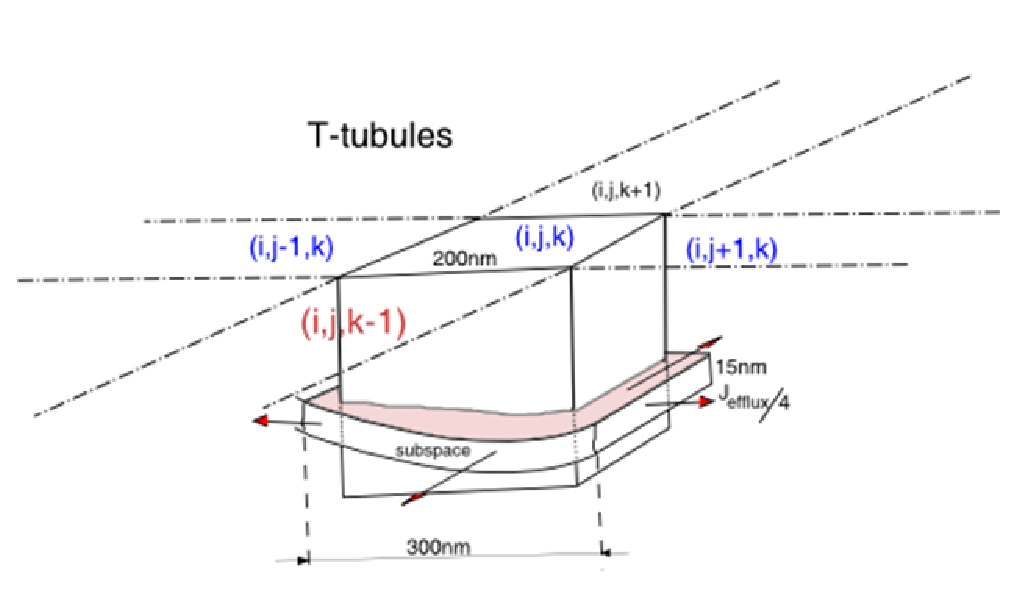
\includegraphics[height=5cm,
    angle=0]{./images/CRU_spatial.eps}}
  \caption{Model of a CRU}
  \label{fig:CRU_spatial}
\end{figure}
 
